%
% Documento: Resultados Esperados
%

\chapter{Resultados Preliminares}

A partir de uma análise sobre qualidade de \textit{software}, métricas de qualidade e fundamentos teóricos do funcionamento do CSS, construiu-se uma pesquisa exploratória, em forma de um questionário, para identificação dos aspectos mais relevantes no processo de manutenção de uma folha de estilo e das características do código fonte que estão relacionadas a sua qualidade.

\section{Construindo o questionário}
Elaborou-se o questionário com os seguintes objetivos:

\begin{itemize}
	\item Identificar os aspectos da linguagem que mais impactam na legibilidade do código;
	\item Identificar os parâmetros que definem qualidade de código no ponto de vista dos entrevistados;
	\item Identificar aspectos mais custosos para manutenção;	
\end{itemize}

A partir da coleta das respostas, pode-se analisar os pesos de cada aspecto de qualidade do código CSS em função da manutenibilidade do estilo. Identificando as maiores ocorrências de efeitos colaterais, definindo quais são as técnicas para manter legibilidade mais utilizadas e quais aspectos de organização do código são mais relevantes.

\begin{figure}[!htb]
	\centering
	\caption{Exemplo de questão aplicada no questionário.}
	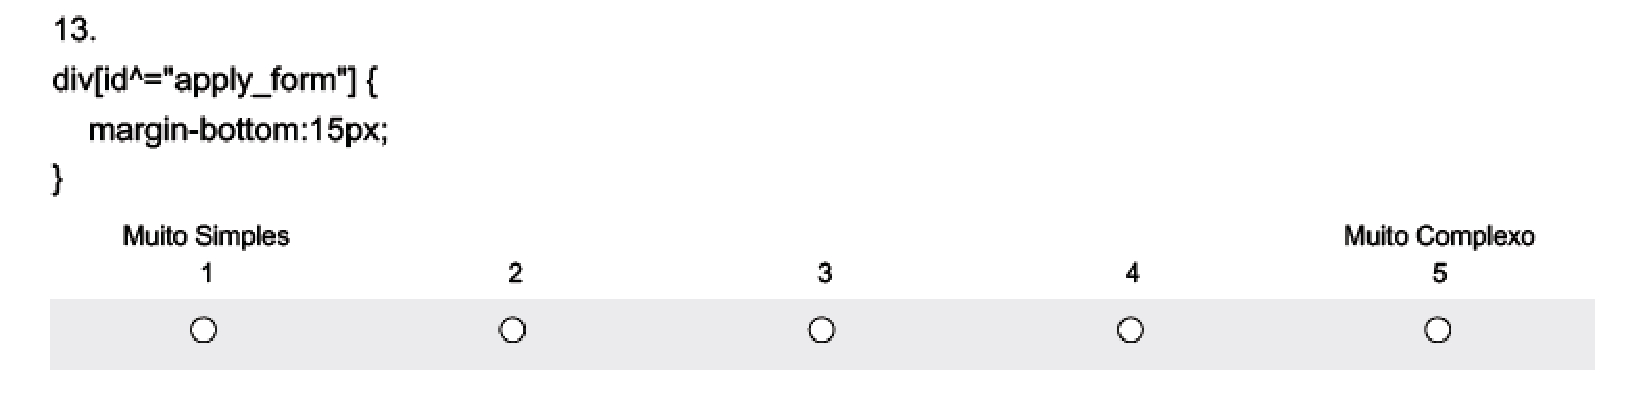
\includegraphics[width=1\textwidth]{./04-figuras/questionario_q13}
	\fonte{próprio autor}
	\label{fig:questionario_q13}
\end{figure}

Viu-se necessária a avaliação da complexidade de alguns aspectos da linguagem, a partir do ponto de vista do profissional, então o questionário (\autoref{chap:apendiceA}) foi construído com uma seção onde é avaliado, com base em um trecho de código (\autoref{fig:questionario_q13}), a dificuldade de se dar manutenção, cada trecho foi elaborado de acordo com um aspecto da linguagem que possam causa algum tipo de complicação. Esses aspectos foram escolhidos de acordo com as ponderações e experiência do autor, com base nos estudos realizados.

A dificuldade atribuída por cada pessoa a um determinado conjunto de regras e propriedades, é subjetiva e depende fortemente da experiência do individuo. Portanto construiu-se o questionário com perguntas visando a classificação do respondente de acordo com o seu nível de conhecimento, a partir dessa classificação será possível ponderar as respostas de acordo com o nível dos respondentes.